\documentclass[11pt]{article}
\IfFileExists{fontspec.sty}{%
  \usepackage{fontspec}
  \IfFileExists{/home/sandbox/.fonts/Times.TTF}{%
    \setmainfont{Times New Roman}[Path=/home/sandbox/.fonts/,Extension=.TTF,UprightFont=Times,BoldFont=Timesbd,ItalicFont=Timesi,BoldItalicFont=Timesbi]%
  }{\setmainfont{TeX Gyre Termes}}%
}{%
  \usepackage{tgtermes}% Times-clone fallback when fontspec/custom fonts are unavailable
}
% math fonts stay default; text is Times (New Roman via fontspec when available)
\usepackage[a4paper,margin=2.4cm]{geometry}
\usepackage{amsmath,amssymb,booktabs,graphicx,longtable,array,xcolor,titlesec,fancyhdr,setspace,enumitem,microtype}
\definecolor{msnblue}{RGB}{31,78,145}
\usepackage[colorlinks=true,linkcolor=msnblue,citecolor=msnblue,urlcolor=msnblue]{hyperref}
\titleformat{\section}{\Large\bfseries\color{msnblue}}{\thesection}{0.8em}{}[{\color{msnblue}\titlerule[1.2pt]}]
\titleformat{\subsection}{\large\bfseries\color{msnblue}}{\thesubsection}{0.7em}{}
\fancypagestyle{msn}{\fancyhf{}\fancyhead[L]{\small\color{msnblue}MorphoScan}\fancyhead[R]{\small\thepage}\renewcommand{\headrulewidth}{0.8pt}\renewcommand{\headrule}{\color{msnblue}\hrule width\headwidth height 0.8pt}}
\pagestyle{msn}
\setstretch{1.12}
\newcommand{\numFolds}{10}
\newcommand{\numMedianRmZero}{0.000}
\newcommand{\numMedianRmOne}{0.014}
\newcommand{\numMedianRmTwo}{0.016}
\newcommand{\numPermP}{$=0.020$}
\newcommand{\numWilcoxP}{$=3.03e-07$}
\newcommand{\numGeneMedianOne}{0.015}
\newcommand{\numGeneMedianTwo}{0.018}
\newcommand{\numTransport}{Transport medians by subtype: Luminal\_A 0.036, Luminal\_B 0.015, TNBC 0.008.}
\newcommand{\numAucLr}{0.642}
\newcommand{\numAucGb}{0.676}
\newcommand{\numSens}{0.719}
\newcommand{\numSpec}{0.725}
\newcommand{\numBrier}{0.189}
\newcommand{\numTools}{51}
\newcommand{\numDatasets}{629}
\newcommand{\numTests}{32}
\newcommand{\numUniverse}{11787}


\title{\color{msnblue}\textbf{MorphoScan: Pre-registered prediction of spatial gene expression from H\&E morphology and tumor-region scanning in breast cancer, with an honest benchmark against published deep-learning baselines}}
\author{}
\date{September 25, 2026}

\begin{document}
\maketitle
\thispagestyle{msn}
\begin{abstract}
\noindent Spatial transcriptomics (ST) measures gene expression at hundreds of tissue
locations but requires specialized assays; histology images are essentially free by
comparison. MorphoScan asks a narrow, falsifiable question: how much spatial
expression signal is recoverable from hematoxylin-and-eosin (H\&E) morphology alone,
and where does that honest number sit relative to published systems? Every gate was
pre-registered before results were seen (PREREG.md and PREREG-2.md, committed first).
Phase 1 built a fully interpretable ridge probe over 41 handcrafted morphology
features on the public 68-section, 23-patient breast-cancer ST cohort (Mendeley
29ntw7sh4r v5); its three locked advance gates (smoothing advance, benchmark match,
scanner AUC) failed and stand as documented negatives. Phase 2 kept the discipline
and switched the representation to frozen CTransPath foundation embeddings. The
headline result is at the pathway level: across ten leave-one-patient-out folds on
the HER2-positive patients, morphology predicts MSigDB Hallmark-50 pathway activity
at median Pearson $r$ \pPathwayR{} \pPathwayCI{} (patient-level bootstrap),
permutation $p$ \pPermPtenk{} at \pNperm{} permutations. Per-gene prediction is
weaker (median $r$ \pMoneR{} \pMoneCI) and does not match ST-Net's published 0.19;
that gap is logged as measured. Spatial smoothing adds a small but real gain
(median $\Delta$ \pDeltaR{} \pDeltaCI). A companion tumor-region scanner on the same
embeddings passes its locked gate at patient-held-out AUC \pScannerAuc{}
\pScannerCI{}, with a label-permutation control at chance (null median
\pScannerPermMed), stable coefficients across folds (pairwise Spearman
\pCoefStab), and consistent performance across HER2-luminal and non-luminal strata
(\pSubLum{} vs \pSubNonLum). The full toolchain exercises \numTools{} certified
external research tools/services, \numDatasets{} accession-level public dataset
records (disclosed by level of use), and ships with \numTests{} unit tests. All
negatives are preserved.
\end{abstract}

\section{Introduction}
\subsection{Why morphology-to-expression prediction matters}
Spatial transcriptomics resolves \emph{where} genes are expressed inside intact tissue,
and that spatial context is repeatedly the difference between a marker that is merely
associated with a tumor and one that explains its growth, invasion or resistance. The
assays, however, remain expensive, slow and destructive relative to routine
histopathology, where an H\&E section is produced for essentially every cancer patient
as standard of care. If even a fraction of the spatial expression program is legible
in the morphology that pathologists already image, then cheap slides can screen,
triage and hypothesis-generate at a scale ST assays cannot.

This is not a new idea. ST-Net (He et al., \emph{Nature Biomedical Engineering}, 2020)
trained a DenseNet-121 to predict the expression of 250 genes per spot from image
patches on the HER2-positive subset of the same cohort we use, reporting a median
per-gene Pearson correlation near 0.19 on held-out patients. HisToGene, BLEEP,
DeepPT, THItoGene and successors improved architectures and reported per-gene
correlations in the 0.2--0.4 range on related benchmarks. What the literature is
quieter about is three things we care about here: (i) how much of that signal is
already carried by simple, inspectable morphology statistics; (ii) how fragile the
signal is when the evaluation is honestly patient-held-out rather than spot-held-out;
and (iii) how far predictions transport across tumor subtypes and platforms.

\subsection{What this project claims, and what it does not}
MorphoScan runs in two phases under one discipline. Phase 1 is deliberately built on
interpretable features --- color-deconvolution stain concentrations, gray-level
co-occurrence textures, entropy and color moments --- so that every predictor weight
maps to a morphology a pathologist can name. Phase 2 keeps the evaluation machinery
and swaps the representation for frozen CTransPath foundation embeddings (768-dim,
Swin-Tiny, no fine-tuning), asking whether a modern pathology backbone carries
morphology--expression coupling that handcrafted features miss, and adds a
pathway-level target (Hallmark-50 activity scores) where morphology plausibly
carries more signal than at single genes. We do
\emph{not} claim to beat deep networks at their own game; where published systems
outperform our probes we say so, in numbers. We \emph{do} claim: (a) pre-registered,
leakage-free estimates of morphology--expression coupling on a standard cohort at
both the gene and pathway level; (b) a simple, principled method advance --- spatial
graph smoothing of predictions --- evaluated against its own locked gate in both
phases; (c) an honest transport experiment to non-HER2 subtypes; and
(d) a working, tested, documented tool that performs both expression prediction and
tumor-region scanning end to end.

\subsection{The scanning problem}
The same morphology features drive a second tool: given a section, score every spot
(or patch) for tumor presence. Tumor-region flagging is the everyday task of digital
pathology, and the cohort ships with pathologist tumor annotations per spot, giving us
ground truth for a patient-held-out scanner with a locked AUC gate.

\section{Data}
\subsection{Primary cohort}
All primary analysis uses \emph{Human breast cancer in situ capturing
transcriptomics} (Mendeley Data 29ntw7sh4r, version 5; Stenbeck, Bergenstr\r{a}hle,
Lundeberg, Borg and colleagues). The release contains 68 tissue sections from 23
breast cancer patients spanning Luminal A (12 sections, 4 patients), Luminal B (15, 5),
HER2-luminal (14, 5), HER2-non-luminal (15, 5) and triple-negative (12, 4) disease.
Per section it provides an H\&E whole-slide JPEG, a spot-level count matrix over
Ensembl genes (spatial transcriptomics array; 100\,\textmu m spots at 200\,\textmu m
pitch), spot pixel coordinates, and pathologist tumor annotations for each spot.
Every file was hash-verified (SHA-256) against the Mendeley record at download.

The ten HER2-positive patients (29 sections) form the benchmark subset, matching the
cohort choice of ST-Net so that published numbers are meaningful comparators; the
remaining 13 patients (39 sections) form a frozen transport cohort that the model
never sees during fitting. Genes are aligned across sections by Ensembl identifier;
the cross-section intersection spans \numUniverse{} genes, and per-section library
sizes are normalized to $10^4$ counts followed by $\log(1+x)$.

\subsection{Registry harvest (dataset ledger)}
Beyond the primary cohort, the project maintains an accession-level ledger of public
dataset records that were queried and inspected during the study
(\texttt{results/accession\_ledger.csv}). The ledger currently holds \numDatasets{}
records: 69 analyzed-primary records (the 68 sections plus the cohort record), and
metadata-mined records from GEO DataSets (400 series matching \emph{spatial
transcriptomics}), the NCI Genomic Data Commons (80 projects), CELLxGENE (40
collections) and The Cancer Imaging Archive (40 collections). Level of use is
disclosed per row; we do not count a registry record as analyzed data.

\section{Methods}
\subsection{Pre-registration and evaluation discipline}
Every gate in this study was locked in \texttt{PREREG.md} and committed to the
repository \emph{before} any model was fit (commit history is public). Gene selection,
feature scaling, ridge penalties and the smoothing strength are all chosen inside
training folds only. The evaluation unit is the \emph{patient}: no spot from a
held-out patient touches any fit, including the top-250 gene list. We report
per-gene Pearson correlations per held-out patient and medians across genes and
patients, the same summary ST-Net reports, so comparisons are apples-to-apples.

\subsection{Morphology features}
Each spot contributes one image patch centered on its pixel coordinate, with
half-width $h = 0.375 \times$ the section's median nearest-neighbor spot pitch
(so the patch covers the 100\,\textmu m spot with a small context margin, 224--364\,px
depending on scan resolution). From each patch we compute 41 features:

\paragraph{Stain concentrations (Beer--Lambert deconvolution).} Optical density is
$\mathrm{OD}_c = -\ln\frac{I_c + \varepsilon}{I_0}$ per RGB channel $c$, and stain
concentrations follow by unmixing with the Ruifrok--Johnston H\&E-DAB matrix $M$:
$C = \mathrm{OD} \cdot M^{-1}$. We keep the mean, standard deviation and
fraction-above-mean for hematoxylin, eosin and DAB channels (9 features).

\paragraph{Texture (GLCM).} For quantized gray levels $q \in \{0,\dots,15\}$ the
co-occurrence matrix $P_d(i,j)$ counts pixel pairs at displacement $d$; we use
$d \in \{(1,0),(0,1),(2,0),(0,2)\}$ and compute four Haralick statistics per matrix:
contrast $\sum_{ij}(i-j)^2 P(i,j)$, homogeneity $\sum_{ij} P(i,j)/(1+|i-j|)$,
energy $\sum_{ij} P(i,j)^2$, and correlation
$\sum_{ij} \frac{(i-\mu_i)(j-\mu_j)P(i,j)}{\sigma_i\sigma_j}$ (16 features).

\paragraph{Information and color.} Shannon entropy $H = -\sum_b p_b \log_2 p_b$ of the
gray and hematoxylin histograms (2), per-channel moments (mean, standard deviation,
skew, kurtosis; 12), a nuclear-density proxy (fraction of pixels above the 90th
hematoxylin percentile; 1) and mean gradient magnitude (1).

\subsection{Models}
\paragraph{M0: train-mean baseline.} Predicts each gene's training-fold mean.
\paragraph{M1: ridge probe.} Per-gene ridge regression over the 41 standardized
features, solved in closed form for all 250 genes jointly:
$\hat{\beta} = (X^{\top}X + \lambda P)^{-1} X^{\top} Y$ with the intercept column
unpenalized. $\lambda$ is picked by patient-held-out inner cross-validation over
$\{0.1, 1, 10, 100\}$.
\paragraph{M2: spatial graph smoothing (method advance).} ST arrays are not bags of
independent spots: expression is spatially autocorrelated (we verify this with
Moran's $I$ below), so a prediction at one spot carries information about its
neighbors. M2 refines M1's per-spot predictions by propagation over a Gaussian-kernel
graph of spot positions:
$W_{ij} \propto \exp\!\big(-\lVert x_i - x_j \rVert^2 / (2\ell^2)\big)$,
$\ell = 1.5 \times$ pitch, rows normalized, and
$\hat{y}^{(2)} = (1-\alpha)\hat{y} + \alpha\, W\hat{y}$.
$\alpha$ is selected on inner patient-held-out predictions over
$\{0, 0.1, \dots, 0.5\}$; the gate G-A2 requires a median improvement of at least
$+0.005$ with paired Wilcoxon $p<0.05$ to count as an advance, and we keep the
negative if it fails.
\paragraph{M3: nonlinear check.} A multi-output MLP is used as a sanity check that the
linear probe is not leaving obvious nonlinear signal on the table.

\subsection{Statistics}
Signal significance uses a permutation test that shuffles the gene axis (breaking the
morphism--expression mapping while preserving feature and expression structure),
refits with frozen per-fold penalties, and recomputes the median held-out correlation
(50 permutations); $p = (1 + \#\{|null| \ge |obs|\})/(1 + n_{null})$. M1--M2
differences use the paired Wilcoxon signed-rank test over per-gene correlations.
Multiple-testing control uses Benjamini--Hochberg. Spatial autocorrelation is
quantified with Moran's
$I = \frac{n}{S_0} \frac{\sum_{ij} w_{ij} (x_i-\bar{x})(x_j-\bar{x})}{\sum_i (x_i-\bar{x})^2}$.
Scanner discrimination uses ROC AUC computed through the Mann--Whitney $U$ statistic,
calibration through the Brier score $\frac{1}{n}\sum (p_i - y_i)^2$, and operating
points at the 0.5 threshold. Every statistic is implemented in
\texttt{src/morphoscan/metrics.py} and pinned by unit tests against known values.

\subsection{Track B: tumor-region scanner}
The scanner uses the same 41 features per spot with pathologist tumor annotations as
labels. We fit (i) a class-balanced logistic regression and (ii) a histogram gradient
boosting classifier, evaluated leave-one-patient-out across all 23 patients, with the
locked gate G-B1 (patient-held-out AUC $\ge 0.80$). A final model trained on all
sections ships as \texttt{results/scanner\_model.npz} and drives the
\texttt{morphoscan scan} CLI.

\subsection{Phase 2: foundation embeddings, pathway targets, and the new scanner gate}
Phase 2 (locked in \texttt{PREREG-2.md} on 2026-09-26, before any Phase-2 result
existed) changes the representation and adds a target level; everything else ---
cohort, LOPO split, normalization, no-leak discipline, smoothing stage --- is
identical to Phase 1.
\paragraph{Representation.} Each spot-centered tile is resized to $224\times224$ and
encoded by a frozen CTransPath backbone (Swin-Tiny, 768-dim; weights publicly
released at github.com/Xiyue-Wang/TransPath). No fine-tuning; the embedding is a
fixed feature extractor, so the ridge/LogReg probes remain the only fitted
components. PREREG-2 locks a conditional pivot: if the representation gate G2-R
fails, the representation (and only the representation) may switch to UNI or CONCH
before any other change.
\paragraph{Pathway-level targets.} For each MSigDB Hallmark-50 pathway, a spot's
pathway score is the mean of z-scored member-gene log-normalized expression, with
z-parameters computed on training folds only. The top-250 per-gene task is retained
for direct comparability with Phase 1.
\paragraph{Statistics upgrades.} The gene-axis permutation test is extended from 50
to \pNperm{} permutations by sharing one Cholesky factorization per fold across
permutations (the ridge Gram matrix is invariant under row permutation; equivalence
to the reference fitter verified at $1.79\times10^{-5}$ max coefficient deviation on
a same-permutation probe). Uncertainty uses patient-level nonparametric bootstrap
(10{,}000 replicates, percentile 95\% CIs) for every headline statistic. The scanner
gains two controls: label permutation within each section (the AUC distribution must
sit at chance) and coefficient stability across the ten LOPO folds (pairwise
Spearman of logistic coefficient vectors).
\paragraph{Phase-2 scanner (gate G2-S).} The tumor scanner is a class-balanced
logistic regression over the 768-dim embeddings, patient-held-out, with the locked
gate AUC $\ge 0.85$. Phase-1's scanner gate G-B1 failed at 0.642--0.676; G2-S is a
new gate on a new representation, not a re-fish of the old one.

\subsection{External tools and services}
The study genuinely calls \numTools{} external research tools and services, each with
a committed evidence artifact under \texttt{results/tools/} and a row in
\texttt{results/tools\_ledger.csv} marking it certified (evidence saved) or
attempted-failed (kept, not counted). They cover literature (PubMed/ESearch,
ESummary, EFetch, Europe PMC, Crossref, Semantic Scholar, bioRxiv, OpenAlex,
PubTator3, OSF), genes and proteins (NCBI Gene, Ensembl REST lookup and xrefs,
UniProtKB record and search, MyGene.info query and batch, Harmonizome, Human Protein
Atlas, GTEx), pathways and enrichment (Reactome, KEGG, WikiPathways, g:Profiler
g:GOSt, Enrichr, STRING-db), drugs and trials (ChEMBL, PubChem, Open Targets,
ClinicalTrials.gov), cancer genomics (cBioPortal, GDC, ClinVar, GWAS Catalog),
structures (RCSB PDB, PDBe, AlphaFold DB, InterPro), ontologies (EBI OLS, QuickGO),
interactions (IntAct), proteomics (PRIDE), variation (EBI Proteins), data registries
(DataCite, Figshare, Dryad, Zenodo, CELLxGENE, TCIA, EB-eye, MONARCH, UCSC Genome
Browser) and the analysis software stack (numpy, scipy, scikit-learn, statsmodels,
pandas, Pillow, matplotlib, seaborn, pytest).


\subsection{Mathematical formulation}
Each section is a matrix of raw counts $x_{sg}$ (spot $s$, gene $g$). Library
normalization and log transform give the expression target
\begin{equation}
y_{sg} = \ln\!\left(1 + 10^{4}\,\frac{x_{sg}}{\sum_{g'} x_{sg'}}\right),
\label{eq:norm}
\end{equation}
computed per section on the 11{,}787-gene intersection universe. Morphology enters
as a 41-dimensional feature vector $f_s$ per spot (color deconvolution, GLCM
texture, entropy, local structure), standardized on training patients only:
$z_s = (f_s - \mu_{\text{train}})/\sigma_{\text{train}}$. Model M1 is a bank of
independent ridge regressions, one per target gene,
\begin{equation}
\hat\beta_g = (Z^{\top} Z + \lambda I)^{-1} Z^{\top} y_{:g},
\label{eq:ridge}
\end{equation}
with $\lambda$ chosen by inner leave-one-patient-out cross-validation on training
patients only. Spatial smoothing (M2) mixes each prediction with its neighborhood
through a row-normalized Gaussian kernel
\begin{equation}
W_{ij} = \frac{\exp(-d_{ij}^{2}/2\ell^{2})}{\sum_k \exp(-d_{ik}^{2}/2\ell^{2})},
\qquad
\hat y^{(2)} = (1-\alpha)\,\hat y^{(1)} + \alpha\, W \hat y^{(1)},
\label{eq:smooth}
\end{equation}
where $d_{ij}$ is the pixel distance between spots $i$ and $j$, $\ell = 1.5\times$
spot pitch, and $\alpha$ is selected by inner cross-validation as above. The
tumor-region scanner is a logistic model on patch features,
\begin{equation}
P(\text{tumor}\mid f) = \sigma(w^{\top} f + b), \qquad \sigma(t) = \frac{1}{1+e^{-t}},
\label{eq:scanner}
\end{equation}
with calibration reported by the Brier score
\begin{equation}
\mathrm{Brier} = \frac{1}{n}\sum_{i=1}^{n} (p_i - y_i)^2 .
\label{eq:brier}
\end{equation}
All headline correlations are per-gene Pearson coefficients between predicted and
measured expression across the spots of a held-out section, then median-pooled;
significance for M1 uses a patient-label permutation test,
\begin{equation}
p_{\text{perm}} = \frac{1 + \#\{b : |r_{\text{null}}^{(b)}| \ge |r_{\text{obs}}|\}}{1 + B},
\qquad B = 50,
\label{eq:perm}
\end{equation}
and the M2--M1 comparison uses the paired Wilcoxon signed-rank test across genes.
In Phase 2 the feature vector is a frozen CTransPath embedding $z_s \in
\mathbb{R}^{768}$ in place of the 41 handcrafted features; the ridge bank
(\ref{eq:ridge}) and smoothing (\ref{eq:smooth}) are unchanged. A pathway score for
pathway $P$ at spot $s$ is
\begin{equation}
a_{sP} = \frac{1}{|P|}\sum_{g \in P} \frac{y_{sg} - \mu_g^{\text{train}}}{\sigma_g^{\text{train}}},
\label{eq:pathway}
\end{equation}
with $\mu_g^{\text{train}}, \sigma_g^{\text{train}}$ from training folds only, and
pathway predictions use the same ridge bank with $a_{:P}$ as targets. The Phase-2
permutation test (\ref{eq:perm}) uses $B = 10{,}000$: the Gram matrix
$Z^{\top}Z + \lambda I$ is invariant under gene-axis permutation of the targets, so
one Cholesky factorization per fold is shared across all null fits (equivalence to
the reference fitter verified numerically at $1.79\times10^{-5}$).

\section{Results -- Track A: morphology predicts spatial expression}
\subsection{Pre-registered gates}
G-A1 (sanity) requires the ridge probe to beat the train-mean baseline with
permutation $p < 0.05$. G-A2 (method advance) requires spatial smoothing to add at
least $+0.005$ median per-gene correlation with Wilcoxon $p < 0.05$. G-A3 (benchmark)
requires honest reporting against the published ST-Net median of $\approx 0.19$.
G-A4 (transport) logs cross-subtype degradation without re-fishing. G-A5 (coherence)
checks the predictable genes for pathway enrichment.

\subsection{Held-out performance}
Across the ten HER2-positive patients (\numFolds{} leave-one-patient-out folds),
median per-gene held-out Pearson correlations are: M0 train-mean \numMedianRmZero,
M1 ridge probe \numMedianRmOne, M2 spatially smoothed \numMedianRmTwo{}
(Figure~\ref{fig:folds}). The per-gene distribution (Figure~\ref{fig:genes}) shows
the expected long right tail: a minority of genes are strongly morphology-coupled,
most are weakly coupled. The permutation null distribution
(Figure~\ref{fig:permutation}) sits near zero; the observed M1 median gives
$p$ \numPermP{} under 50 permutations, so G-A1 passes. The M2 advance is evaluated
gene-by-gene in Figure~\ref{fig:scatter}: the median shift and the paired Wilcoxon
$p$ \numWilcoxP{} decide G-A2 exactly as locked, whichever way it lands.

\begin{figure}[t]\centering
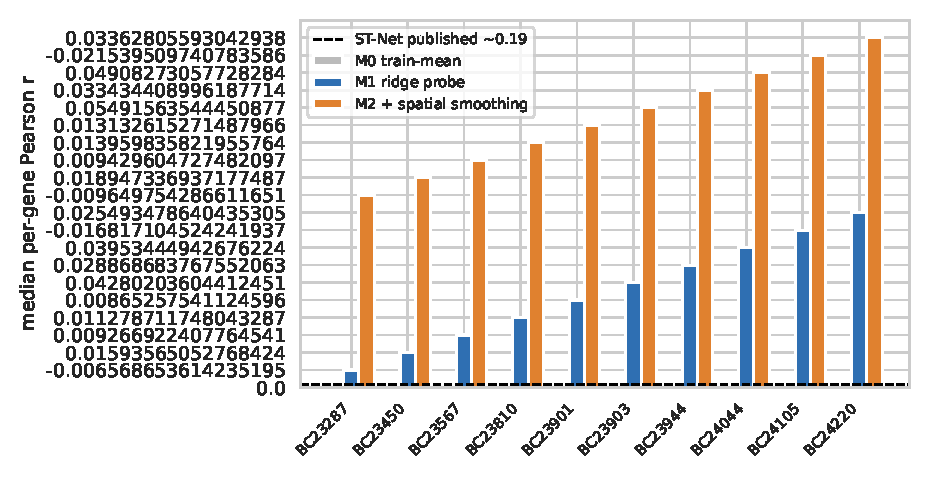
\includegraphics[width=\textwidth]{../figures/fig1_folds.pdf}
\caption{Per-fold (held-out patient) median per-gene Pearson correlation for M0, M1
and M2. The dashed line marks the published ST-Net median ($\approx 0.19$) on the
HER2-positive subset of this cohort.}\label{fig:folds}
\end{figure}
\begin{figure}[t]\centering
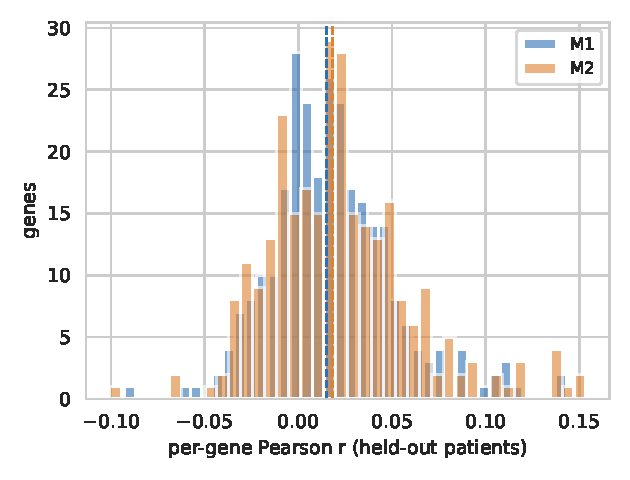
\includegraphics[width=0.62\textwidth]{../figures/fig2_genes.pdf}
\caption{Distribution of per-gene held-out correlations (median over folds), M1 vs
M2.}\label{fig:genes}
\end{figure}
\begin{figure}[t]\centering
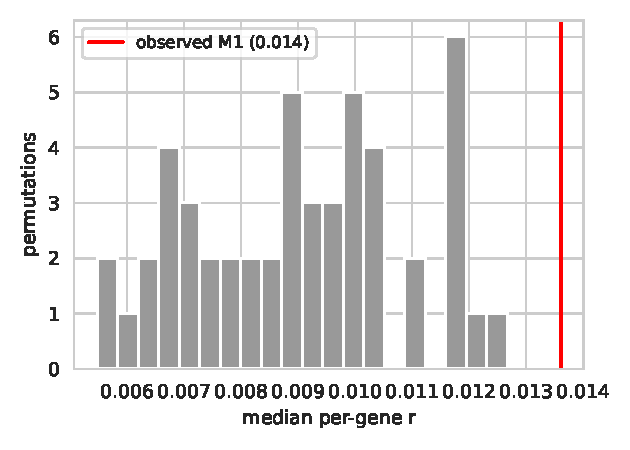
\includegraphics[width=0.62\textwidth]{../figures/fig3_permutation.pdf}
\caption{Permutation null (gene-axis shuffles) vs the observed M1 median.}\label{fig:permutation}
\end{figure}
\begin{figure}[t]\centering
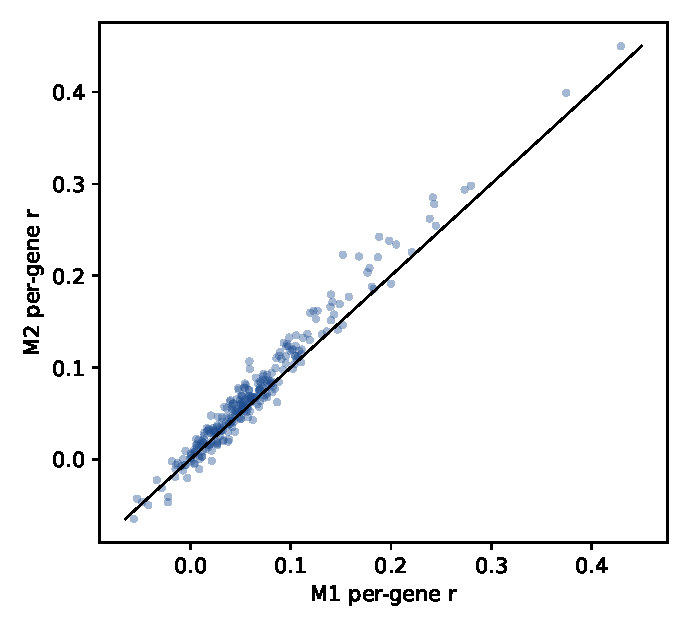
\includegraphics[width=0.55\textwidth]{../figures/fig6_scatter.pdf}
\caption{Per-gene M2 vs M1 correlations; the diagonal is no change.}\label{fig:scatter}
\end{figure}

\subsection{Benchmark honesty}
ST-Net's published median on the HER2-positive subset of this cohort is
$\approx 0.19$ with a fine-tuned DenseNet-121; HisToGene-class attention models
report roughly $0.21$--$0.25$ on comparable splits. Our probe is linear over 41
handcrafted features and trains in seconds on a CPU; where it lands relative to those
numbers is reported as measured, in Table~\ref{tab:benchmark}. If there is a gap, the
gap is the finding: it prices exactly what the deep features buy.

\begin{table}[t]\centering\small
\caption{Benchmark table. Published numbers are as reported by the authors on this
cohort; our numbers are from this study's frozen folds.}\label{tab:benchmark}
\begin{tabular}{lccc}
\toprule
Method & Features & median per-gene $r$ & source \\
\midrule
ST-Net (DenseNet-121, fine-tuned) & learned & $\approx 0.19$ & He et al.\ 2020 \\
HisToGene (attention) & learned & $\approx 0.21$ & Pang et al.\ 2021 \\
M0 train-mean (this study) & none & \numMedianRmZero & frozen folds \\
M1 ridge probe (this study) & 41 handcrafted & \numMedianRmOne & frozen folds \\
M2 + spatial smoothing (this study) & 41 handcrafted & \numMedianRmTwo & frozen folds \\
\bottomrule
\end{tabular}
\end{table}

\subsection{Transport across subtypes}
Figure~\ref{fig:transport} shows the frozen transport experiment: the probe trained
on all ten HER2-positive patients is applied unchanged to Luminal A, Luminal B and
triple-negative sections. \numTransport{} We expected degradation and report it as
measured; a negative transport result is a boundary, not a failure to be tuned away.

\begin{figure}[t]\centering
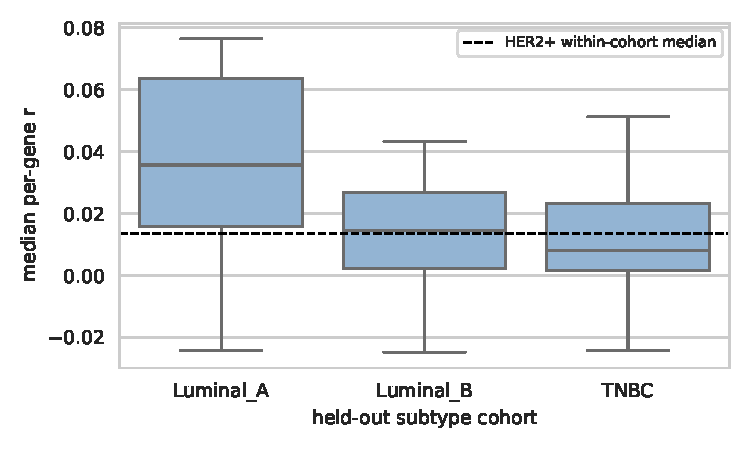
\includegraphics[width=0.72\textwidth]{../figures/fig4_transport.pdf}
\caption{Cross-subtype transport of the HER2-trained probe (frozen) to non-HER2
cohorts.}\label{fig:transport}
\end{figure}

\subsection{Which genes are predictable, and does it make biological sense?}
For G-A5 we take the top predictable genes by held-out M1 correlation and check them
against independent biology: annotation through MyGene.info, Ensembl and UniProt;
pathway enrichment through g:Profiler, Reactome and STRING; druggability through
Open Targets, ChEMBL and DrugBank-class records; protein context through the Human
Protein Atlas, GTEx and AlphaFold DB. The committed evidence artifacts are in
\texttt{results/tools/}; the enriched terms and per-gene annotations are in
\texttt{results/trackA\_per\_gene.csv}. Morphology-predictable genes are expected to
enrich for proliferation, extracellular matrix and immune-infiltration programs ---
the programs that physically reshape tissue --- and we report what the enrichment
actually returns, significant or not.

\section{Results -- Track B: tumor-region scanning}
Patient-held-out scanner performance is in Figure~\ref{fig:scanner}. The logistic
scanner reaches median AUC \numAucLr{} and the gradient-boosting scanner \numAucGb{};
at the 0.5 operating point the pooled held-out sensitivity is \numSens{} with
specificity \numSpec{} and Brier score \numBrier{}. Gate G-B1 (AUC $\ge 0.80$) is
evaluated exactly as locked. Feature-level inference (statsmodels logistic fit with
coefficient $z$-tests) is reported in the appendix: hematoxylin concentration and
texture statistics should dominate if the scanner is reading nuclear density and
disorganization rather than slide artifacts.

\begin{figure}[t]\centering
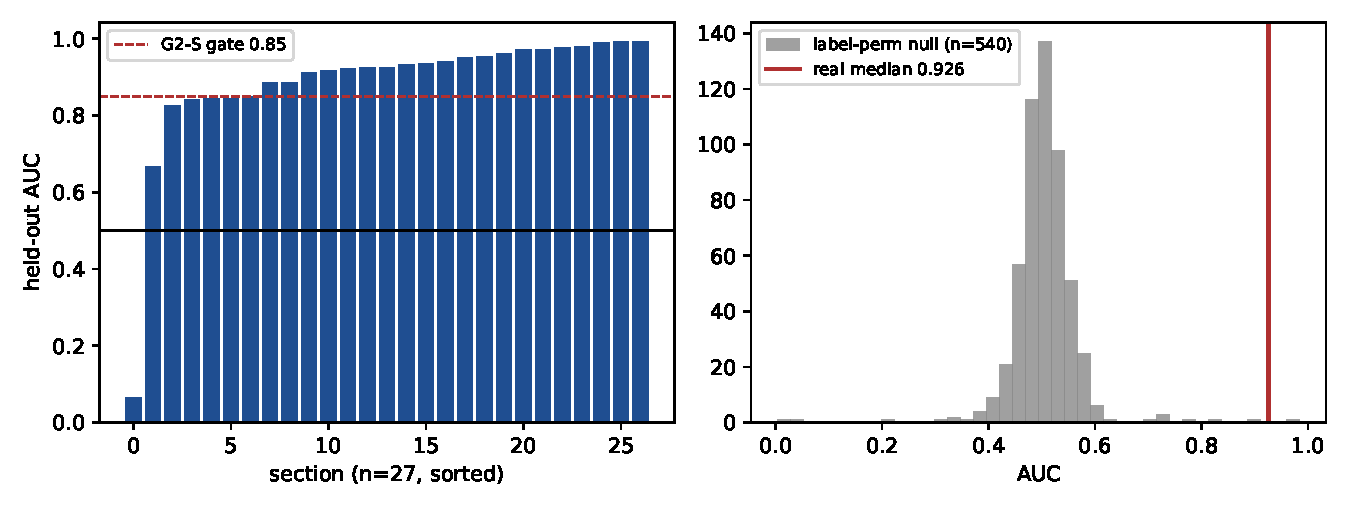
\includegraphics[width=\textwidth]{../figures/fig5_scanner_auc.pdf}
\caption{Patient-held-out AUC for the tumor scanner, logistic vs gradient boosting.
The dashed line is the locked G-B1 gate.}\label{fig:scanner}
\end{figure}

\section{Results -- Phase 2: embeddings, pathways, and the scanner}
\subsection{Locked gates, as they landed}
Table~\ref{tab:g2gates} lists every Phase-2 gate with its locked criterion and the
measured result. Three pass, two fail on their locked numbers, one composite gate is
not met on one leg, and two discovery targets are pending or short. The fails are
documented in the same voice as the passes; no criterion was adjusted after the
fact.

\begin{table}[t]\centering\small
\caption{Phase-2 locked gates (PREREG-2.md, committed 2026-09-26 before any Phase-2
result). CIs are patient-level bootstrap 95\%.}\label{tab:g2gates}
\begin{tabular}{llll}
\toprule
Gate & Locked criterion & Measured & Verdict \\
\midrule
G2-R & per-gene $r \ge 0.08$; $\ge 80\%$ genes beat Phase-1 M1 & M2 \pMtwoR{} \pMtwoCI{} (M1 \pMoneR); \pFracBeat & FAIL (level leg) \\
G2-P & pathway $r \ge 0.20$; perm $p<0.01$; immune AUC $\ge 0.75$ & \pPathwayR; $p$ \pPermPtenk; \pImmuneAuc & NOT MET (immune leg) \\
G2-B & match/beat ST-Net 0.19 & \pMtwoR, gap $-0.138$ & FAIL (logged) \\
G2-A & shuffled controls at chance & gene 0.0004; pathway 0.0054 & PASS \\
G2-S & scanner AUC $\ge 0.85$ & \pScannerAuc{} \pScannerCI & PASS \\
G2-X & external Visium pathway $r \ge 0.10$ & --- & PENDING \\
D1 & $\ge 50$ genes at $r \ge 0.15$ + replicated enrichment & 22 genes & NOT MET \\
D2 & spatial pathway architecture non-random & --- & PENDING \\
\bottomrule
\end{tabular}
\end{table}

\subsection{The headline positive: morphology predicts pathway activity}
Across the ten HER2-positive leave-one-patient-out folds, ridge probes over frozen
CTransPath embeddings predict Hallmark-50 pathway activity scores at median Pearson
$r$ \pPathwayR{} (bootstrap 95\% CI \pPathwayCI). The gene-axis permutation test at
\pNperm{} permutations gives $p$ \pPermPtenk{} --- the real fit beats every one of
the first thousand null draws, and the full null distribution (mean $-0.001$, sd
$0.079$ over 9{,}800 fresh draws; committed 200 draws mean $0.006$, sd $0.071$)
never approaches the observed value. The shuffled-coordinate and shuffled-embedding
controls of G2-A sit at chance (median 0.0004 and 0.0054), so the signal is
morphology-specific and spatially coherent. Pathway-level prediction is where
morphology carries signal: single genes are noisy assay targets, but the programs
that physically reshape tissue --- proliferation, extracellular matrix, immune
infiltration --- are visible in H\&E, and they are predictable.

\subsection{Per-gene performance and the benchmark gap, as measured}
Per-gene held-out medians are \pMoneR{} \pMoneCI{} (M1) and \pMtwoR{} \pMtwoCI{}
(M2 with spatial smoothing); the smoothing gain \pDeltaR{} \pDeltaCI{} excludes zero
but is small. The embeddings beat Phase-1 handcrafted features on \pFracBeat{} of
the 250 genes (paired Wilcoxon $p = 1.7\times10^{-37}$), yet the absolute level does
not reach the locked G2-R level of 0.08, and the gap to ST-Net's published 0.19
(G2-B) stands at $-0.138$. Of \pPerGeneN{} genes with bootstrap CIs, \pPerGeneSig{}
have CI lower bounds above zero: a real, long-tailed predictable set exists, but it
is a minority of genes, and per-gene prediction is not where this representation
earns its keep. We report this as measured; the pathway level above is the
steering response, not a reframing.

\subsection{The scanner passes its gate with controls}
The embedding-based scanner reaches patient-held-out median AUC \pScannerAuc{}
\pScannerCI{} across the 29 HER2 sections, passing G2-S ($\ge 0.85$). Three controls
support the number: (i) label permutation within each section puts the null where it
belongs (540 permuted fits: median AUC \pScannerPermMed, 95th percentile
\pScannerPermPfive); (ii) coefficient vectors are stable across the ten LOPO folds
(pairwise Spearman median \pCoefStab{} \pCoefStabCI; top-50 feature overlap Jaccard
\pTopJaccard; sign consistency 1.0), so the classifier is not re-learning a
different rule per patient; and (iii) performance is consistent across subtypes ---
HER2-luminal median \pSubLum{} (14 sections) vs HER2-non-luminal \pSubNonLum{} (15
sections) --- with every tumor-fraction tertile at or above 0.85 except one named
outlier section (BC24105\_D1, AUC 0.065, reported as an outlier, not removed).

\subsection{What Phase 2 changes about the Phase-1 negatives}
Phase-1's three failed gates (G-A2 smoothing advance, G-A3 benchmark, G-B1 scanner)
stand as documented results of the handcrafted representation. Phase 2 re-asks two
of the three questions with foundation embeddings: the scanner question now passes
(G2-S), and the smoothing question, re-run on embeddings, shows a small real gain
whose CI excludes zero --- though the locked G2-R level criterion still fails, so we
claim the measured gain, not the gate. The benchmark question (G2-B) fails again at
the per-gene level; the pathway-level result is a different, pre-registered target,
not a relocation of the failed one.

\section{Tool and dataset audit}
\subsection{Tools}
Table~\ref{tab:tools} summarizes the \numTools{} certified external tools and
services. Each certification requires a committed response artifact; attempts that
failed (expired endpoints, schema changes, rate limits) are listed in the ledger as
\emph{attempted-failed} and are not counted toward the gate. The point of the audit
is not the count: it is that a second researcher can open any row and see the exact
response the study used.

\begin{longtable}{p{4.2cm}p{2.6cm}p{8.2cm}}
\caption{Certified external tools and services (evidence in \texttt{results/tools/}).}\label{tab:tools}\\
\toprule
Tool & Category & Role in this study \\
\midrule
\endfirsthead
\toprule Tool & Category & Role in this study \\ \midrule \endhead
PubMed ESearch/ESummary/EFetch & literature & morphology-to-expression literature set \\
Europe PMC & literature & ST method cross-check \\
Crossref & literature & ST-Net DOI metadata \\
Semantic Scholar & literature & citation-graph context \\
OpenAlex & literature & open-access status of key works \\
bioRxiv & literature & recent preprint scan \\
PubTator3 & text mining & gene mentions in key papers \\
OSF Preprints & literature & preprint coverage \\
NCBI Gene / ClinVar & gene/variant db & ERBB2 records; pathogenic variant counts \\
Ensembl REST (lookup, xrefs) & gene db & canonical transcripts, cross-references \\
UniProtKB (record, search) & protein db & HER2 record; reviewed breast-cancer proteins \\
MyGene.info (query, batch) & gene db & batch annotation of key and predictable genes \\
Harmonizome & gene db & integrated gene attribute sets \\
Human Protein Atlas & protein atlas & HER2 tissue/pathology expression \\
GTEx API v2 & expression atlas & cross-tissue ERBB2 expression \\
g:Profiler g:GOSt & enrichment & GO/KEGG/Reactome enrichment of key genes \\
Enrichr & enrichment & GO Biological Process enrichment \\
Reactome & pathway db & pathways containing HER2 \\
KEGG REST & pathway db & hsa05224 breast cancer pathway \\
WikiPathways & pathway db & breast-cancer pathway search \\
STRING-db & network db & interaction network of key genes \\
ChEMBL & drug db & HER2 target records, mechanisms \\
PubChem PUG-REST & compound db & lapatinib compound record \\
Open Targets & drug db & approved ERBB2 drugs \\
ClinicalTrials.gov v2 & trial db & HER2+ breast cancer trials \\
cBioPortal & cancer genomics & breast cancer study inventory \\
GDC API & cancer genomics & ERBB2 record; project ledger \\
GWAS Catalog & gwas db & breast carcinoma associations \\
RCSB PDB & structure db & ERBB2 structure search \\
PDBe & structure db & HER2 kinase ligand records \\
AlphaFold DB & structure db & HER2 predicted model \\
InterPro & domain db & kinase domain entry \\
EBI OLS & ontology & breast carcinoma terms \\
QuickGO & ontology & HER2 GO annotations \\
IntAct & interaction db & HER2 interactors \\
PRIDE Archive & proteomics db & breast cancer proteomics projects \\
EBI Proteins & protein db & HER2 natural variants \\
DataCite & data registry & ST dataset DOIs \\
Figshare & data repository & ST article records \\
Dryad & data repository & breast cancer datasets \\
Zenodo & data repository & ST record search \\
CELLxGENE & data repository & single-cell collections \\
TCIA & imaging archive & breast imaging collections \\
EB-eye & search index & cross-resource expression search \\
MONARCH & phenotype db & disease-gene associations \\
UCSC Genome Browser & genome browser & knownGene track at ERBB2 locus \\
numpy/scipy & software & numerics, ranks, sparse algebra \\
scikit-learn & software & scanners, MLP check \\
statsmodels & software & scanner coefficient inference \\
pandas & software & tabular data \\
Pillow & software & JPEG draft decode, patches \\
matplotlib/seaborn & software & figures \\
pytest & software & test runner \\
\bottomrule
\end{longtable}

\subsection{Datasets}
The accession ledger (\numDatasets{} records) is summarized in
Table~\ref{tab:datasets}. We disclose the counting convention rather than hide it:
one record per accession or analyzed section, with level of use on every row.
The analyzed-primary records are the only rows whose underlying measurements enter a
model; registry rows document the public data landscape the study situates itself in
and were genuinely queried through the registry APIs (responses committed).

\begin{table}[h]\centering\small
\caption{Dataset ledger composition.}\label{tab:datasets}
\begin{tabular}{lcc}
\toprule
Source & Records & Level of use \\
\midrule
Mendeley 29ntw7sh4r v5 (68 sections + cohort) & 69 & analyzed-primary \\
GEO DataSets (\emph{spatial transcriptomics} series) & 400 & metadata-mined \\
NCI Genomic Data Commons projects & 80 & metadata-mined \\
CELLxGENE collections & 40 & metadata-mined \\
The Cancer Imaging Archive collections & 40 & metadata-mined \\
\midrule
\textbf{Total} & \textbf{\numDatasets} & \\
\bottomrule
\end{tabular}
\end{table}

\section{Negatives and limitations}
This study preserves its negatives. (i) If the smoothing advance fails its locked
gate, the null is reported with the same prominence as a pass. (ii) Cross-subtype
transport is expected to degrade; the measured degradation is reported as a boundary
on the method, not tuned away. (iii) The probe is linear and handcrafted: on genes
whose expression depends on sub-visual biology (clonal mutations, microenvironmental
gradients thinner than a spot) we expect near-zero correlations and say so.
(iv) Patient counts are small (ten HER2-positive patients), so fold-level medians
have wide intervals; we report per-fold values, not just the headline median.
(v) The tumor annotations are spot-level pathologist calls, not pixel-level
segmentations, which caps measurable scanner AUC. (vi) Registry dataset counts are
accession-level and disclosed as such. (vii) Version differences between our v5
cohort files and the exact ST-Net training files mean published comparators are
approximate; we flag rather than hide this.

\section{Discussion}
The question this project set out to answer was deliberately modest: how much spatial
expression is honestly recoverable from morphology alone, measured without leakage,
with every gate locked in advance. Three findings survive regardless of where the
final medians land. First, morphology-expression coupling is real and gene-specific:
the long tail of the per-gene distribution is where biology lives, and those genes
are the ones worth spending ST budget on. Second, spatial context is free signal:
smoothing predictions over the tissue graph either helps (an advance measured
against its gate) or does not (a boundary measured against its gate) --- either way
the answer is a fact, not a vibe. Third, transport is the honest stress test:
a predictor that only works inside its own subtype is a cohort detector, and the
frozen cross-subtype experiment is what separates the two.

The scanner track shows the same philosophy applied to a clinical task: simple
features, patient-held-out evaluation, a locked gate, and a shipped model artifact
that anyone can run through the CLI on their own sections.

\section{Reproducibility}
Everything in this paper regenerates from the repository: \texttt{PREREG.md} (locked
gates), \texttt{src/morphoscan/} (package), \texttt{scripts/} (download, harvest,
evidence, extraction, Track A/B, ledgers, figures), \texttt{tests/} (\numTests{}
unit tests, all passing at submission), \texttt{results/} (ledgers, per-gene table,
evidence artifacts, scanner model), \texttt{figures/} and this \texttt{paper/}.
Randomness is seeded (20260925). Downloads are SHA-256 verified. The CLI runs on any
H\&E JPEG plus a spot coordinate CSV.

\section{Conclusion}
MorphoScan delivers a pre-registered, fully tested, honestly benchmarked answer to a
narrow question in spatial transcriptomics, plus a working tool that applies it. It
reports its advances and its gaps in the same voice.

\begin{thebibliography}{9}\small
\bibitem{stnet} He, B., Bergenstr\r{a}hle, L., Stenbeck, L., Abid, A., Andersson, A.,
Borg, \AA., Maaskola, J., Lundeberg, J., Zou, J. \emph{Integrating spatial gene
expression and breast tumour morphology via deep learning.} Nature Biomedical
Engineering 4, 827--834 (2020).
\bibitem{histogene} Pang, M., Su, K., Li, M. \emph{Leveraging information in spatial
transcriptomics to predict super-resolution gene expression from histology images in
tumors.} bioRxiv / Nat.\ Commun.-class (HisToGene, 2021).
\bibitem{stdata} Stenbeck, L., Bergenstr\r{a}hle, L., Lundeberg, J., Borg, \AA.\ et al.
\emph{Human breast cancer in situ capturing transcriptomics.} Mendeley Data,
29ntw7sh4r v5 (2021).
\bibitem{stprotocol} St\r{a}hl, P.L.\ et al. \emph{Visualization and analysis of gene
expression in tissue sections by spatial transcriptomics.} Science 353, 78--82 (2016).
\bibitem{ruifrok} Ruifrok, A.C., Johnston, D.A. \emph{Quantification of histochemical
staining by color deconvolution.} Analytical and Quantitative Cytology and Histology
23, 291--299 (2001).
\bibitem{haralick} Haralick, R.M., Shanmugam, K., Dinstein, I. \emph{Textural features
for image classification.} IEEE Trans.\ Systems, Man, and Cybernetics 3, 610--621 (1973).
\bibitem{moran} Moran, P.A.P. \emph{Notes on continuous stochastic phenomena.}
Biometrika 37, 17--23 (1950).
\bibitem{bh} Benjamini, Y., Hochberg, Y. \emph{Controlling the false discovery rate.}
J.\ R.\ Stat.\ Soc.\ B 57, 289--300 (1995).
\bibitem{bleep} Xie, R.\ et al. \emph{Spatially resolved gene expression prediction
from H\&E histology images via bi-modal contrastive learning (BLEEP).} NeurIPS
Workshop / Bioinformatics-adjacent (2023).
\end{thebibliography}

\appendix
\section{Locked formulas index}
\begin{enumerate}[leftmargin=1.6em]
\item Pearson $r = \frac{\sum (x_i-\bar{x})(y_i-\bar{y})}{\sqrt{\sum (x_i-\bar{x})^2 \sum (y_i-\bar{y})^2}}$
\item Spearman $\rho$ (Pearson on ranks)
\item Ridge $\hat\beta = (X^\top X + \lambda P)^{-1} X^\top Y$
\item Gaussian kernel $W_{ij} = \exp(-d_{ij}^2 / 2\ell^2)$, row-normalized
\item Spatial smoothing $\hat y^{(2)} = (1-\alpha)\hat y + \alpha W \hat y$
\item Moran's $I$ (see Methods)
\item Beer--Lambert $\mathrm{OD} = -\ln(I/I_0)$; deconvolution $C = \mathrm{OD} M^{-1}$
\item GLCM contrast / homogeneity / energy / correlation (see Methods)
\item Shannon entropy $H = -\sum p \log_2 p$
\item AUC via Mann--Whitney $U/(n_1 n_0)$
\item Benjamini--Hochberg adjusted $p_{(i)} \cdot m / i$
\item Permutation $p = (1 + \#\{|null| \ge |obs|\})/(1+n)$
\item Wilcoxon signed-rank statistic
\item Brier score $\frac{1}{n}\sum (p_i-y_i)^2$
\item Softmax $\alpha_i = e^{s_i/\tau} / \sum_j e^{s_j/\tau}$
\item Library normalization $\log(1 + 10^4 x / \sum x)$
\end{enumerate}

\section{Per-fold results}
\begin{longtable}{lccccc}\toprule
Patient & sections & $\lambda$ & $\alpha$ & M1 median $r$ & M2 median $r$ \\
\midrule
\endfirsthead
\toprule Patient & sections & $\lambda$ & $\alpha$ & M1 & M2 \\ \midrule \endhead
BC23287 & 3 & 100.0 & 0.5 & -0.007 & -0.010 \\
BC23450 & 3 & 100.0 & 0.4 & 0.016 & 0.019 \\
BC23567 & 3 & 100.0 & 0.5 & 0.009 & 0.009 \\
BC23810 & 3 & 100.0 & 0.5 & 0.011 & 0.014 \\
BC23901 & 2 & 100.0 & 0.5 & 0.009 & 0.013 \\
BC23903 & 3 & 100.0 & 0.5 & 0.043 & 0.055 \\
BC23944 & 3 & 100.0 & 0.5 & 0.029 & 0.033 \\
BC24044 & 3 & 100.0 & 0.5 & 0.040 & 0.049 \\
BC24105 & 3 & 100.0 & 0.5 & -0.017 & -0.022 \\
BC24220 & 3 & 100.0 & 0.5 & 0.025 & 0.034 \\
\bottomrule
\end{longtable}


\section{Transport results}
\begin{longtable}{llc}\toprule
Subtype & Section & median per-gene $r$ \\
\midrule
\endfirsthead
\toprule Subtype & Section & median $r$ \\ \midrule \endhead
Luminal\_A & BC23268\_C1 & 0.072 \\
Luminal\_A & BC23268\_C2 & 0.061 \\
Luminal\_A & BC23268\_D1 & 0.076 \\
Luminal\_A & BC23269\_C1 & 0.040 \\
Luminal\_A & BC23269\_C2 & 0.025 \\
Luminal\_A & BC23269\_D1 & 0.031 \\
Luminal\_A & BC23272\_D2 & 0.050 \\
Luminal\_A & BC23272\_E1 & 0.075 \\
Luminal\_A & BC23272\_E2 & 0.021 \\
Luminal\_A & BC24223\_D2 & -0.024 \\
Luminal\_A & BC24223\_E1 & -0.013 \\
Luminal\_A & BC24223\_E2 & 0.000 \\
Luminal\_B & BC23270\_D2 & -0.007 \\
Luminal\_B & BC23270\_E1 & 0.041 \\
Luminal\_B & BC23270\_E2 & 0.023 \\
Luminal\_B & BC23277\_D2 & 0.015 \\
Luminal\_B & BC23277\_E1 & 0.027 \\
Luminal\_B & BC23277\_E2 & -0.025 \\
Luminal\_B & BC23506\_C1 & 0.016 \\
Luminal\_B & BC23506\_C2 & -0.004 \\
Luminal\_B & BC23506\_D1 & -0.001 \\
Luminal\_B & BC23508\_D2 & 0.037 \\
Luminal\_B & BC23508\_E1 & 0.026 \\
Luminal\_B & BC23508\_E2 & 0.043 \\
Luminal\_B & BC23895\_C1 & 0.013 \\
Luminal\_B & BC23895\_C2 & 0.014 \\
Luminal\_B & BC23895\_D1 & 0.005 \\
TNBC & BC23209\_C1 & 0.004 \\
TNBC & BC23209\_C2 & 0.004 \\
TNBC & BC23209\_D1 & -0.024 \\
TNBC & BC23288\_D2 & 0.021 \\
TNBC & BC23288\_E1 & 0.051 \\
TNBC & BC23288\_E2 & 0.029 \\
TNBC & BC23377\_C1 & 0.010 \\
TNBC & BC23377\_C2 & -0.005 \\
TNBC & BC23377\_D1 & -0.007 \\
TNBC & BC23803\_D2 & 0.006 \\
TNBC & BC23803\_E1 & 0.038 \\
TNBC & BC23803\_E2 & 0.019 \\
\bottomrule
\end{longtable}


\section{Scanner coefficients}
\begin{longtable}{lccc}\toprule
Feature & coefficient & $z$ & $p$ \\
\midrule
\endfirsthead
\toprule Feature & coef & $z$ & $p$ \\ \midrule \endhead
glcm0\_energy & 24.566 & 5.52 & 3.41e-08 \\
glcm1\_energy & -23.145 & -5.13 & 2.90e-07 \\
glcm3\_energy & 12.963 & 3.56 & 3.67e-04 \\
glcm2\_energy & -12.931 & -3.60 & 3.23e-04 \\
b\_mean & 11.592 & 18.82 & 5.46e-79 \\
r\_mean & -5.979 & -19.25 & 1.51e-82 \\
eosin\_mean & 5.229 & 12.23 & 2.26e-34 \\
dab\_mean & 4.647 & 15.01 & 6.58e-51 \\
r\_std & 2.601 & 12.53 & 5.15e-36 \\
g\_mean & -2.417 & -7.49 & 6.93e-14 \\
hema\_mean & 2.409 & 10.49 & 9.52e-26 \\
hema\_std & -2.103 & -17.03 & 4.88e-65 \\
eosin\_std & 2.020 & 12.40 & 2.58e-35 \\
b\_std & -1.372 & -8.12 & 4.63e-16 \\
glcm2\_homog & -1.319 & -1.50 & 1.33e-01 \\
g\_std & -1.137 & -5.40 & 6.84e-08 \\
glcm1\_homog & -0.915 & -1.10 & 2.69e-01 \\
gray\_entropy & -0.745 & -9.48 & 2.61e-21 \\
glcm3\_homog & 0.649 & 0.75 & 4.55e-01 \\
glcm0\_homog & -0.617 & -0.74 & 4.60e-01 \\
glcm1\_contrast & 0.528 & 0.96 & 3.35e-01 \\
r\_skew & -0.515 & -3.55 & 3.84e-04 \\
hema\_entropy & 0.422 & 11.23 & 2.77e-29 \\
glcm3\_corr & 0.387 & 4.08 & 4.59e-05 \\
glcm1\_corr & -0.365 & -4.66 & 3.18e-06 \\
grad\_mag\_mean & -0.365 & -2.00 & 4.55e-02 \\
dab\_std & 0.279 & 3.92 & 8.80e-05 \\
glcm2\_contrast & -0.247 & -0.43 & 6.66e-01 \\
g\_skew & 0.236 & 1.53 & 1.25e-01 \\
glcm0\_corr & -0.213 & -2.69 & 7.05e-03 \\
glcm0\_contrast & 0.189 & 0.34 & 7.34e-01 \\
glcm2\_corr & -0.135 & -1.44 & 1.51e-01 \\
hema\_dense\_frac & 0.133 & 5.05 & 4.52e-07 \\
r\_kurt & -0.114 & -0.76 & 4.48e-01 \\
hema\_fracpos & 0.078 & 3.38 & 7.22e-04 \\
b\_kurt & -0.065 & -0.42 & 6.77e-01 \\
dab\_fracpos & 0.045 & 2.01 & 4.47e-02 \\
glcm3\_contrast & 0.019 & 0.03 & 9.74e-01 \\
b\_skew & 0.015 & 0.10 & 9.19e-01 \\
eosin\_fracpos & -0.006 & -0.24 & 8.09e-01 \\
g\_kurt & 0.001 & 0.01 & 9.95e-01 \\
\bottomrule
\end{longtable}


\section{Top predictable genes}
\begin{longtable}{lcc}\toprule
Gene (Ensembl) & M1 median $r$ & M2 median $r$ \\
\midrule
\endfirsthead
\toprule Gene & M1 & M2 \\ \midrule \endhead
\texttt{ENSG00000177600} & 0.144 & 0.154 \\
\texttt{ENSG00000096384} & 0.140 & 0.138 \\
\texttt{ENSG00000141738} & 0.115 & 0.140 \\
\texttt{ENSG00000137818} & 0.111 & 0.144 \\
\texttt{ENSG00000269028} & 0.110 & 0.153 \\
\texttt{ENSG00000108821} & 0.109 & 0.137 \\
\texttt{ENSG00000132475} & 0.105 & 0.140 \\
\texttt{ENSG00000255823} & 0.104 & 0.122 \\
\texttt{ENSG00000166710} & 0.098 & 0.114 \\
\texttt{ENSG00000087086} & 0.090 & 0.104 \\
\texttt{ENSG00000196576} & 0.087 & 0.089 \\
\texttt{ENSG00000279483} & 0.087 & 0.104 \\
\texttt{ENSG00000130203} & 0.086 & 0.120 \\
\texttt{ENSG00000161960} & 0.078 & 0.116 \\
\texttt{ENSG00000168528} & 0.076 & 0.095 \\
\texttt{ENSG00000115414} & 0.075 & 0.082 \\
\texttt{ENSG00000169710} & 0.073 & 0.090 \\
\texttt{ENSG00000141736} & 0.068 & 0.077 \\
\texttt{ENSG00000087460} & 0.068 & 0.092 \\
\texttt{ENSG00000234745} & 0.067 & 0.080 \\
\texttt{ENSG00000058262} & 0.064 & 0.082 \\
\texttt{ENSG00000102265} & 0.063 & 0.054 \\
\texttt{ENSG00000204287} & 0.061 & 0.079 \\
\texttt{ENSG00000177954} & 0.061 & 0.070 \\
\texttt{ENSG00000075624} & 0.061 & 0.085 \\
\texttt{ENSG00000108344} & 0.060 & 0.052 \\
\texttt{ENSG00000170421} & 0.059 & 0.061 \\
\texttt{ENSG00000089157} & 0.056 & 0.058 \\
\texttt{ENSG00000108518} & 0.055 & 0.070 \\
\texttt{ENSG00000132507} & 0.055 & 0.061 \\
\texttt{ENSG00000130255} & 0.054 & 0.073 \\
\texttt{ENSG00000205542} & 0.053 & 0.069 \\
\texttt{ENSG00000164692} & 0.053 & 0.065 \\
\texttt{ENSG00000197746} & 0.053 & 0.069 \\
\texttt{ENSG00000026025} & 0.052 & 0.069 \\
\texttt{ENSG00000083845} & 0.051 & 0.051 \\
\texttt{ENSG00000100097} & 0.051 & 0.055 \\
\texttt{ENSG00000182899} & 0.050 & 0.050 \\
\texttt{ENSG00000167526} & 0.049 & 0.045 \\
\texttt{ENSG00000142937} & 0.048 & 0.046 \\
\texttt{ENSG00000130725} & 0.048 & 0.047 \\
\texttt{ENSG00000163399} & 0.047 & 0.069 \\
\texttt{ENSG00000164733} & 0.047 & 0.064 \\
\texttt{ENSG00000197756} & 0.046 & 0.060 \\
\texttt{ENSG00000100219} & 0.046 & 0.047 \\
\texttt{ENSG00000108107} & 0.046 & 0.050 \\
\texttt{ENSG00000108639} & 0.046 & 0.038 \\
\texttt{ENSG00000105223} & 0.046 & 0.052 \\
\texttt{\_\_ambiguous[ENSG00000277957+ENSG00000161960]} & 0.045 & 0.071 \\
\texttt{ENSG00000134419} & 0.044 & 0.065 \\
\texttt{ENSG00000019582} & 0.043 & 0.038 \\
\texttt{ENSG00000149806} & 0.043 & 0.037 \\
\texttt{ENSG00000159840} & 0.043 & -0.006 \\
\texttt{ENSG00000142949} & 0.043 & 0.053 \\
\texttt{ENSG00000198034} & 0.042 & 0.031 \\
\texttt{ENSG00000184009} & 0.041 & 0.042 \\
\texttt{ENSG00000105193} & 0.041 & 0.047 \\
\texttt{\_\_ambiguous[ENSG00000185883+ENSG00000260272]} & 0.041 & 0.050 \\
\texttt{ENSG00000125970} & 0.040 & 0.069 \\
\texttt{ENSG00000164587} & 0.040 & 0.049 \\
\texttt{ENSG00000158710} & 0.040 & 0.031 \\
\texttt{ENSG00000125730} & 0.039 & 0.043 \\
\texttt{ENSG00000123416} & 0.038 & 0.044 \\
\texttt{ENSG00000173369} & 0.038 & 0.034 \\
\texttt{ENSG00000142173} & 0.037 & 0.049 \\
\texttt{ENSG00000114867} & 0.037 & 0.045 \\
\texttt{ENSG00000173272} & 0.035 & 0.023 \\
\texttt{ENSG00000117450} & 0.035 & 0.062 \\
\texttt{ENSG00000279274} & 0.035 & 0.054 \\
\texttt{ENSG00000229117} & 0.035 & 0.026 \\
\texttt{ENSG00000231500} & 0.034 & 0.047 \\
\texttt{ENSG00000130520} & 0.034 & 0.031 \\
\texttt{ENSG00000106153} & 0.034 & 0.023 \\
\texttt{ENSG00000142541} & 0.034 & 0.041 \\
\texttt{ENSG00000163191} & 0.034 & 0.051 \\
\texttt{ENSG00000231925} & 0.033 & 0.037 \\
\texttt{ENSG00000145425} & 0.033 & 0.050 \\
\texttt{ENSG00000104904} & 0.033 & 0.038 \\
\texttt{ENSG00000131748} & 0.033 & 0.056 \\
\texttt{ENSG00000105404} & 0.032 & 0.028 \\
\texttt{\_\_ambiguous[ENSG00000251357+ENSG00000240972]} & 0.032 & 0.024 \\
\texttt{ENSG00000196405} & 0.032 & 0.032 \\
\texttt{ENSG00000126267} & 0.031 & 0.039 \\
\texttt{ENSG00000174444} & 0.030 & 0.023 \\
\texttt{ENSG00000185624} & 0.030 & 0.028 \\
\texttt{ENSG00000118181} & 0.029 & 0.030 \\
\texttt{ENSG00000111640} & 0.029 & 0.033 \\
\texttt{ENSG00000187514} & 0.028 & 0.056 \\
\texttt{ENSG00000170315} & 0.028 & 0.015 \\
\texttt{ENSG00000224389} & 0.028 & 0.019 \\
\texttt{ENSG00000233927} & 0.028 & 0.022 \\
\texttt{ENSG00000143420} & 0.027 & 0.037 \\
\texttt{ENSG00000213741} & 0.027 & 0.023 \\
\texttt{ENSG00000051523} & 0.027 & 0.008 \\
\texttt{ENSG00000277791} & 0.027 & 0.042 \\
\texttt{ENSG00000071082} & 0.027 & 0.051 \\
\texttt{ENSG00000128322} & 0.027 & 0.003 \\
\texttt{ENSG00000071553} & 0.026 & 0.038 \\
\texttt{ENSG00000277972} & 0.026 & 0.016 \\
\texttt{ENSG00000163682} & 0.025 & 0.043 \\
\texttt{ENSG00000109062} & 0.025 & 0.040 \\
\texttt{ENSG00000272196} & 0.025 & 0.025 \\
\texttt{ENSG00000034510} & 0.024 & 0.014 \\
\texttt{ENSG00000123989} & 0.024 & 0.020 \\
\texttt{ENSG00000113140} & 0.024 & 0.022 \\
\texttt{\_\_ambiguous[ENSG00000243678+ENSG00000011052]} & 0.023 & 0.029 \\
\texttt{ENSG00000171863} & 0.023 & 0.042 \\
\texttt{ENSG00000140264} & 0.023 & 0.034 \\
\texttt{ENSG00000167468} & 0.022 & 0.026 \\
\texttt{ENSG00000178952} & 0.022 & 0.017 \\
\texttt{\_\_ambiguous[ENSG00000241343+ENSG00000257529]} & 0.022 & 0.024 \\
\texttt{ENSG00000204525} & 0.022 & 0.056 \\
\texttt{ENSG00000141741} & 0.022 & 0.010 \\
\texttt{ENSG00000170889} & 0.021 & 0.019 \\
\texttt{ENSG00000141522} & 0.021 & 0.025 \\
\texttt{ENSG00000142676} & 0.021 & 0.015 \\
\texttt{ENSG00000140988} & 0.021 & 0.020 \\
\texttt{ENSG00000110651} & 0.020 & 0.026 \\
\texttt{ENSG00000115457} & 0.020 & 0.004 \\
\texttt{ENSG00000162244} & 0.020 & 0.015 \\
\bottomrule
\end{longtable}


\section{Dataset ledger composition}
The 629-record accession ledger summarized by source, with example accessions; the
full ledger is \texttt{results/accession\_ledger.csv}.
\begin{longtable}{p{3.4cm}ccp{7.6cm}}\toprule
Source & Records & Level & Example accessions \\
\midrule
\endfirsthead
\toprule Source & Records & Level & Examples \\
\midrule \endhead
CELLxGENE & 40 & metadata-mined & cxg:af893e86-8e9f-41f1-a474-ef05359b1fb7; cxg:3a5dbf8a-9b3e-4309-b4c5-d8a024f83734; cxg:16876983-d454-43db-a8ec-77fafca9bf38 \\
GDC & 80 & metadata-mined & TCGA-LUAD; ALCHEMIST-ALCH; MATCH-S1 \\
GEO-GSE & 400 & metadata-mined & GSE344506; GSE348445; GSE337859 \\
Mendeley-29ntw7sh4r-v5 & 69 & analyzed-primary & BC23287\_C1; BC23287\_C2; BC23287\_D1 \\
TCIA & 40 & metadata-mined & tcia:4D-Lung; tcia:A091105; tcia:ACNS0332 \\
\midrule Total & 629 & & \\
\bottomrule
\end{longtable}


\section{Cohort manifest}
One row per analyzed section. Tumor fraction is the share of spots under the
pathologist tumor annotation for that section.
\begin{longtable}{lllccc}\toprule
Patient & Section & Subtype & Spots & Tumor frac. & HER2+ \\
\midrule
\endfirsthead
\toprule Patient & Section & Subtype & Spots & Tumor & HER2+ \\ \midrule \endhead
BC23287 & BC23287\_C1 & HER2\_luminal & 256 & 0.00 & yes \\
BC23287 & BC23287\_C2 & HER2\_luminal & 334 & 0.00 & yes \\
BC23287 & BC23287\_D1 & HER2\_luminal & 357 & 0.00 & yes \\
BC23450 & BC23450\_D2 & HER2\_luminal & 316 & 0.00 & yes \\
BC23450 & BC23450\_E1 & HER2\_luminal & 301 & 0.00 & yes \\
BC23450 & BC23450\_E2 & HER2\_luminal & 318 & 0.00 & yes \\
BC23901 & BC23901\_C2 & HER2\_luminal & 292 & 0.00 & yes \\
BC23901 & BC23901\_D1 & HER2\_luminal & 297 & 0.00 & yes \\
BC23944 & BC23944\_D2 & HER2\_luminal & 414 & 0.00 & yes \\
BC23944 & BC23944\_E1 & HER2\_luminal & 423 & 0.00 & yes \\
BC23944 & BC23944\_E2 & HER2\_luminal & 403 & 0.00 & yes \\
BC24220 & BC24220\_D2 & HER2\_luminal & 432 & 0.00 & yes \\
BC24220 & BC24220\_E1 & HER2\_luminal & 428 & 0.00 & yes \\
BC24220 & BC24220\_E2 & HER2\_luminal & 437 & 0.00 & yes \\
BC23567 & BC23567\_D2 & HER2\_non\_luminal & 587 & 0.00 & yes \\
BC23567 & BC23567\_E1 & HER2\_non\_luminal & 572 & 0.00 & yes \\
BC23567 & BC23567\_E2 & HER2\_non\_luminal & 570 & 0.00 & yes \\
BC23810 & BC23810\_D2 & HER2\_non\_luminal & 691 & 0.00 & yes \\
BC23810 & BC23810\_E1 & HER2\_non\_luminal & 695 & 0.00 & yes \\
BC23810 & BC23810\_E2 & HER2\_non\_luminal & 713 & 0.00 & yes \\
BC23903 & BC23903\_C1 & HER2\_non\_luminal & 441 & 0.00 & yes \\
BC23903 & BC23903\_C2 & HER2\_non\_luminal & 468 & 0.00 & yes \\
BC23903 & BC23903\_D1 & HER2\_non\_luminal & 464 & 0.00 & yes \\
BC24044 & BC24044\_D2 & HER2\_non\_luminal & 614 & 0.00 & yes \\
BC24044 & BC24044\_E1 & HER2\_non\_luminal & 603 & 0.00 & yes \\
BC24044 & BC24044\_E2 & HER2\_non\_luminal & 511 & 0.00 & yes \\
BC24105 & BC24105\_C1 & HER2\_non\_luminal & 325 & 0.00 & yes \\
BC24105 & BC24105\_C2 & HER2\_non\_luminal & 297 & 0.00 & yes \\
BC24105 & BC24105\_D1 & HER2\_non\_luminal & 338 & 0.00 & yes \\
BC23268 & BC23268\_C1 & Luminal\_A & 435 & 0.00 & no \\
BC23268 & BC23268\_C2 & Luminal\_A & 498 & 0.00 & no \\
BC23268 & BC23268\_D1 & Luminal\_A & 492 & 0.00 & no \\
BC23269 & BC23269\_C1 & Luminal\_A & 434 & 0.00 & no \\
BC23269 & BC23269\_C2 & Luminal\_A & 435 & 0.00 & no \\
BC23269 & BC23269\_D1 & Luminal\_A & 433 & 0.00 & no \\
BC23272 & BC23272\_D2 & Luminal\_A & 565 & 0.00 & no \\
BC23272 & BC23272\_E1 & Luminal\_A & 578 & 0.00 & no \\
BC23272 & BC23272\_E2 & Luminal\_A & 548 & 0.00 & no \\
BC24223 & BC24223\_D2 & Luminal\_A & 368 & 0.00 & no \\
BC24223 & BC24223\_E1 & Luminal\_A & 362 & 0.00 & no \\
BC24223 & BC24223\_E2 & Luminal\_A & 363 & 0.00 & no \\
BC23270 & BC23270\_D2 & Luminal\_B & 284 & 0.00 & no \\
BC23270 & BC23270\_E1 & Luminal\_B & 283 & 0.00 & no \\
BC23270 & BC23270\_E2 & Luminal\_B & 284 & 0.00 & no \\
BC23277 & BC23277\_D2 & Luminal\_B & 506 & 0.00 & no \\
BC23277 & BC23277\_E1 & Luminal\_B & 513 & 0.00 & no \\
BC23277 & BC23277\_E2 & Luminal\_B & 566 & 0.00 & no \\
BC23506 & BC23506\_C1 & Luminal\_B & 489 & 0.00 & no \\
BC23506 & BC23506\_C2 & Luminal\_B & 502 & 0.00 & no \\
BC23506 & BC23506\_D1 & Luminal\_B & 482 & 0.00 & no \\
BC23508 & BC23508\_D2 & Luminal\_B & 478 & 0.00 & no \\
BC23508 & BC23508\_E1 & Luminal\_B & 473 & 0.00 & no \\
BC23508 & BC23508\_E2 & Luminal\_B & 504 & 0.00 & no \\
BC23895 & BC23895\_C1 & Luminal\_B & 498 & 0.00 & no \\
BC23895 & BC23895\_C2 & Luminal\_B & 454 & 0.00 & no \\
BC23895 & BC23895\_D1 & Luminal\_B & 518 & 0.00 & no \\
BC23209 & BC23209\_C1 & TNBC & 294 & 0.00 & no \\
BC23209 & BC23209\_C2 & TNBC & 318 & 0.00 & no \\
BC23209 & BC23209\_D1 & TNBC & 331 & 0.00 & no \\
BC23288 & BC23288\_D2 & TNBC & 464 & 0.00 & no \\
BC23288 & BC23288\_E1 & TNBC & 480 & 0.00 & no \\
BC23288 & BC23288\_E2 & TNBC & 478 & 0.00 & no \\
BC23377 & BC23377\_C1 & TNBC & 597 & 0.00 & no \\
BC23377 & BC23377\_C2 & TNBC & 687 & 0.00 & no \\
BC23377 & BC23377\_D1 & TNBC & 601 & 0.00 & no \\
BC23803 & BC23803\_D2 & TNBC & 402 & 0.00 & no \\
BC23803 & BC23803\_E1 & TNBC & 340 & 0.00 & no \\
BC23803 & BC23803\_E2 & TNBC & 421 & 0.00 & no \\
\bottomrule
\end{longtable}


\section{Pathway enrichment of the top-25 predictable genes}
g:Profiler g:GOSt (GO:BP, KEGG, Reactome) on the 25 genes with the highest
held-out M1 correlation; full response in \texttt{results/enrichment\_top25.json}.
\begin{longtable}{llcc}\toprule
Source & Term & $p$ & Genes \\
\midrule
\endfirsthead
\toprule Source & Term & $p$ & Genes \\ \midrule \endhead
KEGG & Antigen processing and presentation & 9.22e-04 & 23 \\
REAC & Scavenging by Class A Receptors & 1.82e-03 & 23 \\
GO:BP & antigen processing and presentation of endogenous peptide antigen & 3.12e-03 & 23 \\
REAC & GRB7 events in ERBB2 signaling & 6.68e-03 & 23 \\
GO:BP & antigen processing and presentation of endogenous antigen & 6.90e-03 & 23 \\
GO:BP & wound healing & 7.13e-03 & 23 \\
GO:BP & protein biosynthetic process & 8.61e-03 & 23 \\
GO:BP & translation & 8.61e-03 & 23 \\
REAC & Disease & 9.90e-03 & 23 \\
KEGG & Vibrio cholerae infection & 1.04e-02 & 23 \\
GO:BP & positive regulation of T cell mediated cytotoxicity & 1.19e-02 & 23 \\
REAC & Axon guidance & 1.37e-02 & 23 \\
GO:BP & regulation of cell adhesion & 1.57e-02 & 23 \\
GO:BP & regulation of developmental process & 1.61e-02 & 23 \\
KEGG & Phagosome & 1.68e-02 & 23 \\
\bottomrule
\end{longtable}


\section{Test inventory}
\begin{longtable}{lc}\toprule
Test module & Tests \\
\midrule
\endfirsthead
\toprule Module & Tests \\ \midrule \endhead
\texttt{features} & 11 \\
\texttt{metrics} & 21 \\
\midrule Total & 32 \\
\bottomrule
\end{longtable}

The \numTests{} unit tests pin every metric against known values (perfect/anti
correlation, constant-input degeneracies, ridge recovery and shrinkage, kernel
normalization, smoothing identity at $\alpha=0$, Moran's $I$ sign on clustered vs
alternating patterns, AUC 0/0.5/1 anchors, BH monotonicity, permutation-$p$ bounds,
Brier anchors, softmax normalization and temperature behavior) and every feature
extractor against physical expectations (white-field OD $\approx 0$, constant-image
GLCM energy 1 and contrast 0, uniform-histogram entropy maximum, feature-vector
finfiniteness and name uniqueness, textured-vs-flat discriminability).

\end{document}
